\documentclass[tikz,border=10pt]{standalone}
\usepackage{tikz}
\usepackage{amsmath}
\usetikzlibrary{arrows.meta, shapes.geometric, positioning, calc}

\definecolor{nodeblue}{RGB}{80,100,160}
\definecolor{nodepurple}{RGB}{140,100,180}
\definecolor{nodered}{RGB}{210,50,50}

\begin{document}
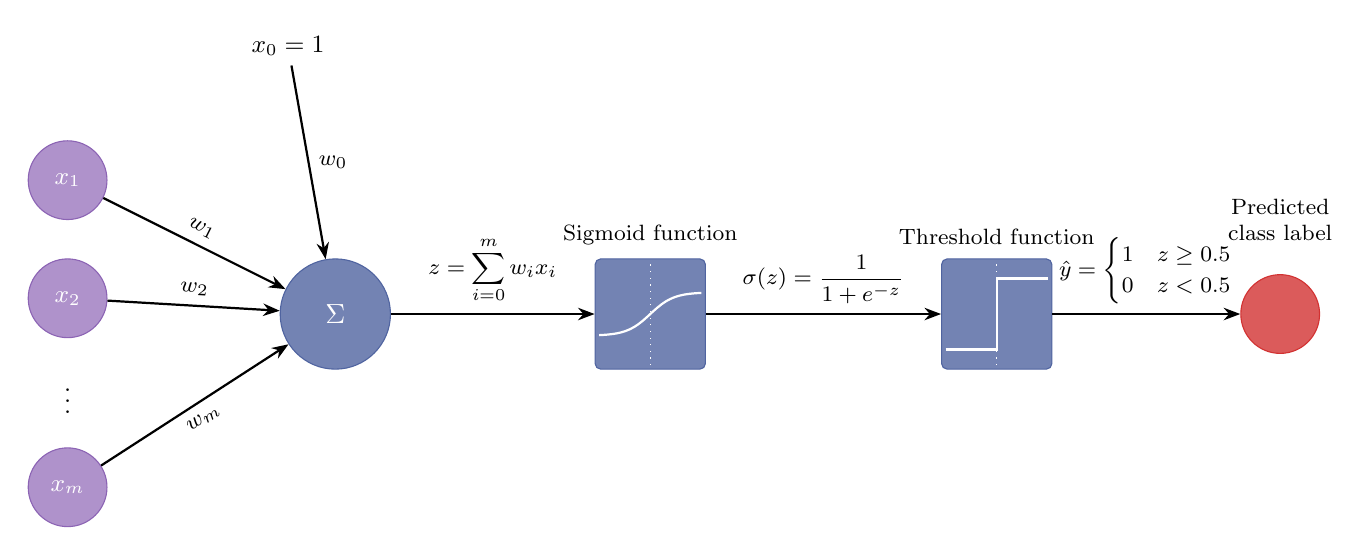
\begin{tikzpicture}[
  every node/.style={font=\small},
  inputnode/.style={circle, draw=nodepurple, fill=nodepurple!70, minimum size=1cm, text=white, font=\small},
  sumnode/.style={circle, draw=nodeblue, fill=nodeblue!80, minimum size=1.4cm, text=white, font=\normalsize},
  funcnode/.style={rectangle, draw=nodeblue, fill=nodeblue!80, minimum width=1.4cm, minimum height=1.4cm, text=white, rounded corners=2pt},
  outputnode/.style={circle, draw=nodered, fill=nodered!80, minimum size=1cm},
  arr/.style={-{Stealth[length=6pt]}, thick},
]

%% Input nodes
\node[inputnode] (x1) at (0, 2.5)   {$x_1$};
\node[inputnode] (x2) at (0, 1.0)   {$x_2$};
\node            (xd) at (0, -0.2)  {\vdots};
\node[inputnode] (xm) at (0, -1.4)  {$x_m$};

%% Bias input
\node (bias) at (2.8, 4.2) {$x_0 = 1$};

%% Summation node
\node[sumnode] (sum) at (3.4, 0.8) {$\Sigma$};

%% Draw input arrows with weights
\draw[arr] (x1) -- node[above, sloped, font=\footnotesize] {$w_1$} (sum);
\draw[arr] (x2) -- node[above, sloped, font=\footnotesize] {$w_2$} (sum);
\draw[arr] (xm) -- node[below, sloped, font=\footnotesize] {$w_m$} (sum);

%% Bias arrow
\draw[arr] (bias) -- node[right, font=\footnotesize] {$w_0$} (sum);

%% Sigmoid node — draw S-curve inside
\node[funcnode] (sigmoid) at (7.4, 0.8) {};
\node[above=0.05cm of sigmoid, font=\footnotesize] {Sigmoid function};
% S-curve in sigmoid box
\begin{scope}
  \clip (6.75, 0.1) rectangle (8.05, 1.5);
  \draw[white, thick, domain=-3:3, samples=40]
    plot ({7.4 + \x * 0.37}, {0.8 + 0.55 * (1/(1+exp(-2.5*\x)) - 0.5)});
\end{scope}
% vertical dotted midline
\draw[white, dotted] (7.4, 0.15) -- (7.4, 1.45);

%% Formula on sum->sigmoid arrow
\draw[arr] (sum) -- node[above, font=\footnotesize] {$z = \displaystyle\sum_{i=0}^{m} w_i x_i$} (sigmoid);

%% Threshold node
\node[funcnode] (thresh) at (11.8, 0.8) {};
\node[above=0.05cm of thresh, font=\footnotesize] {Threshold function};
% Step curve in threshold box
\draw[white, thick] (11.15, 0.35) -- (11.8, 0.35) -- (11.8, 1.25) -- (12.45, 1.25);
\draw[white, dotted] (11.8, 0.15) -- (11.8, 1.45);

%% Sigmoid formula label on arrow
\draw[arr] (sigmoid) -- node[above, font=\footnotesize] {$\sigma(z) = \dfrac{1}{1+e^{-z}}$} (thresh);

%% Output node
\node[outputnode] (out) at (15.4, 0.8) {};
\node[above=0.3cm of out, font=\footnotesize, align=center] {Predicted\\class label};

%% Threshold formula
\draw[arr] (thresh) -- node[above, font=\footnotesize] {
  $\hat{y} = \begin{cases} 1 & z \geq 0.5 \\ 0 & z < 0.5 \end{cases}$
} (out);

\end{tikzpicture}
\end{document}
